\documentclass[aspectratio=169]{beamer}

\usepackage[english]{babel}
\usepackage{microtype}
\usepackage{graphicx}
\usepackage[utf8]{inputenc}
\usepackage{amssymb,amsmath}
\usepackage{resizegather}
\usepackage{ulem}
\usepackage{epsfig}
\usepackage{color}
\usepackage{contour }
\usepackage{colortbl}
\usepackage{mystyl}
\usepackage[style=phys,articletitle=false,maxnames=4,minnames=3]{biblatex}
\bibliography{databank}
\usepackage[font=small]{caption}
\usepackage{chemfig}
\usepackage{multimedia}
% \usepackage{animation}
\usepackage{units}
\usepackage{upgreek}
\usepackage{algorithmicx}
\usepackage{algpseudocode}
\usepackage{epigraph}
\usepackage{tipa}
\usepackage{amsthm}
\usepackage{amscd}
\usepackage{wasysym}
\usepackage{subcaption}
\usepackage{soul}
\usepackage{tikz}
\def\checkmark{\tikz\fill[scale=0.4](0,.35) -- (.25,0) -- (1,.7) -- (.25,.15) -- cycle;}

\usepackage{setspace}
\newcommand{\leftcumulant}{{\langle\langle}}
\newcommand{\rightcumulant}{{\rangle\rangle}}

% Variable width example block
\newenvironment<>{varexampleblock}[2][0.9\textwidth]{%
  \setlength{\textwidth}{#1}%
  \setlength{\linewidth}{\textwidth}%
  \begin{actionenv}#3%
    \def\insertblocktitle{#2}%
    \par%
    \setbeamercolor{local structure}{parent=example text}%
    \usebeamertemplate{block example begin}}
  {\par%
    \usebeamertemplate{block example end}%
  \end{actionenv}
}

\graphicspath{{../figures/}}
\usetheme{Luebeck}
\usecolortheme{own}

\captionsetup[subfigure]{labelformat=empty}

\titlegraphic{
  \vspace{-2\baselineskip}
  \begin{columns}
    \begin{column}{0.16\textwidth}
      \begin{figure}
        \centering
        
\includegraphics[width=0.75\textwidth]{schmidt_logo}
      \end{figure}

    \end{column}
    \begin{column}{0.65\textwidth}
      \centering
      \vspace{0.5\baselineskip}
      \centering
      \begin{figure}
        \centering
        % 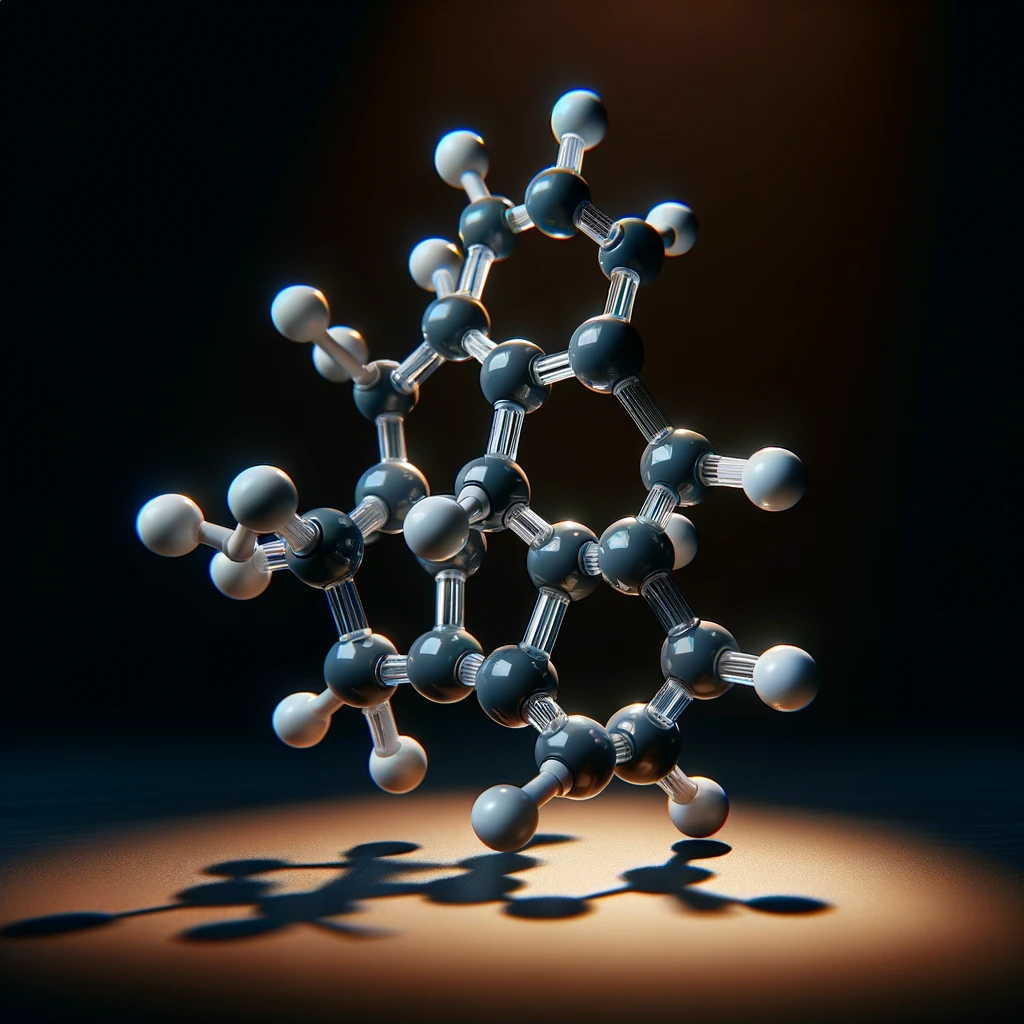
\includegraphics[width=0.25\textwidth]{image}
      \end{figure}
    \end{column}
    \begin{column}{0.16\textwidth}
      \begin{figure}
        \centering
        \includegraphics[width=0.75\textwidth]{uchicago}
      \end{figure}
    \end{column}
  \end{columns}
  \vfill
}

\title{Welcome to the AI+Science Hackathon}
% \author[{
\includegraphics[height=0.95em]{favicon} Ludwig Schneider (he/him)}]{Ludwig Schneider}
\institute{Eric and Wendy Schmidt AI-Postdoctoral Fellowship\\A Schmidt Sciences Program\\University of Chicago}


\begin{document}

\frame{\titlepage\thispagestyle{empty}}
\addtocounter{framenumber}{-1}


% \section*{Introduction}
% \begin{frame}
%   \frametitle{ad}
% \end{frame}


\section{Hackathon Progression}
\begin{frame}
  \frametitle{Day 1: Excitement}
  \begin{columns}
    \begin{column}{0.5\textwidth}
    \begin{itemize}
    \item get to know each other
    \item get to know your mentor
    \item brain storm model ideas
    \item pick a tech stack
    \item build a data pipeline
    \end{itemize}
  \end{column}
  \begin{column}{0.5\textwidth}
    \begin{figure}
      
\includegraphics[width=0.9\textwidth]{day1}
    \end{figure}
  \end{column}
  \end{columns}
\end{frame}

\begin{frame}
  \frametitle{Day 2: Valley of Despair}
  \begin{columns}
    \begin{column}{0.5\textwidth}
      \begin{itemize}
      \item your first ideas didn't work
      \item the excitement is wearing off
      \item brain storm and select most promising idea
      \item iterate and build new models
      \item train new models over night
      \end{itemize}
    \end{column}
    \begin{column}{0.5\textwidth}
    \begin{figure}
      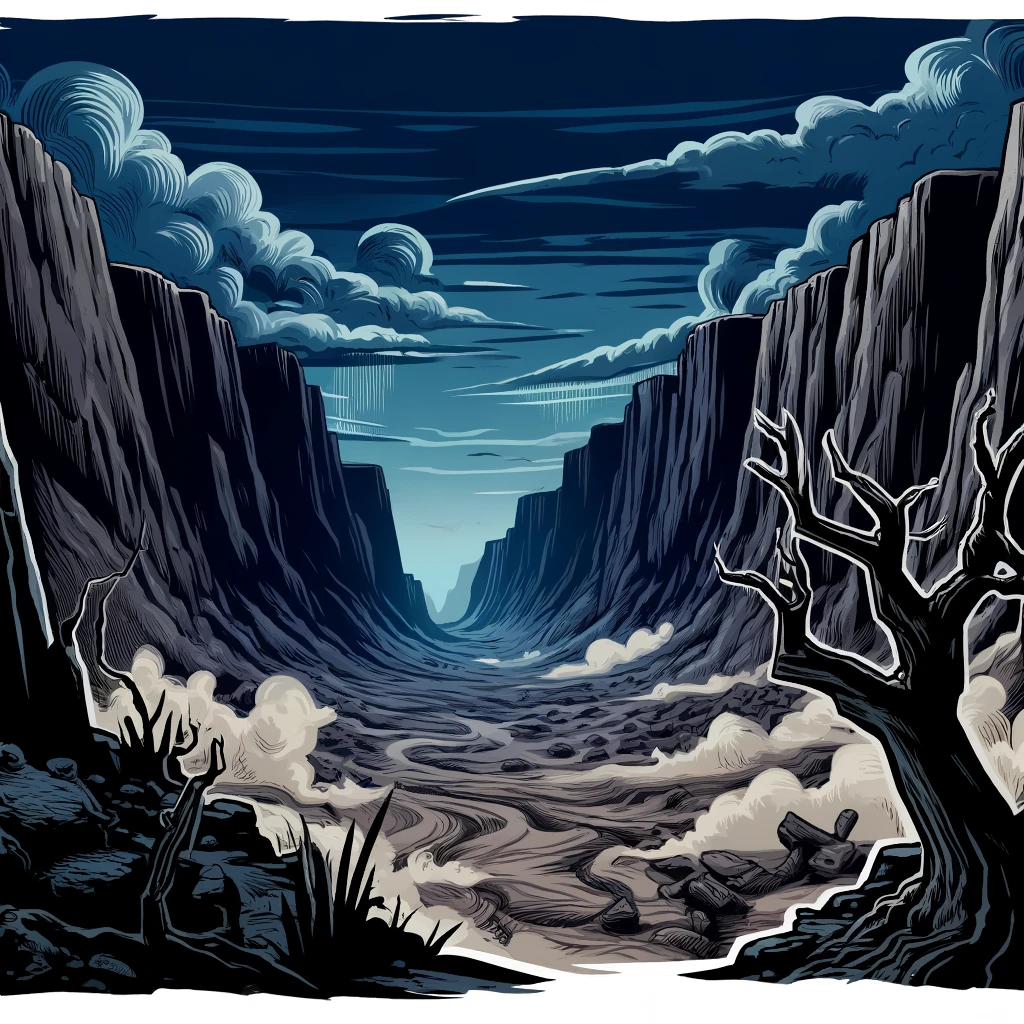
\includegraphics[width=0.9\textwidth]{day2}
    \end{figure}
    \end{column}
  \end{columns}
\end{frame}
\begin{frame}
  \frametitle{Day 3: Seeing the Light}

  \begin{columns}
    \begin{column}{0.5\textwidth}
  \begin{itemize}
  \item your models worked over night!
  \item you can actually see how you solve this!
  \item iterate on your models
  \item optimize your hyper parameters
  \item prepare final training over night
  \end{itemize}
\end{column}
    \begin{column}{0.5\textwidth}
    \begin{figure}
      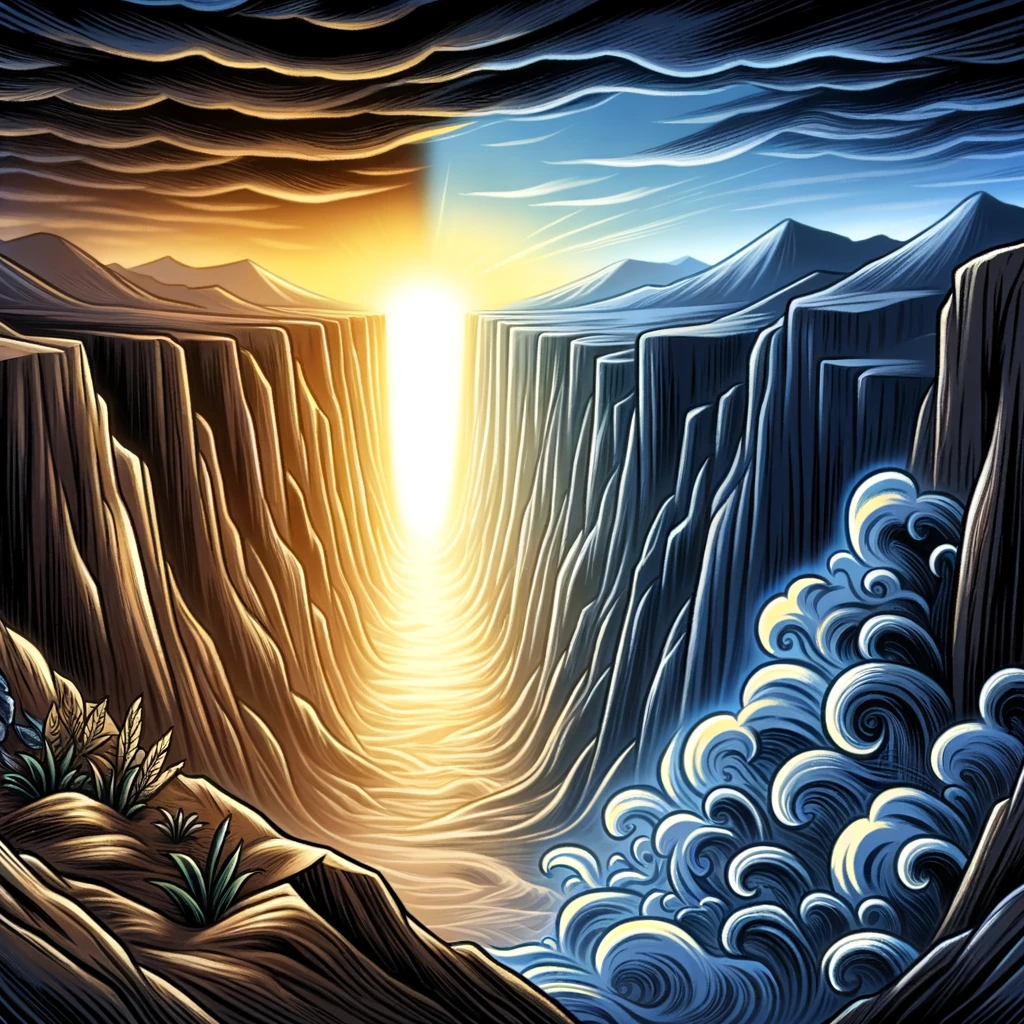
\includegraphics[width=0.9\textwidth]{day3}
    \end{figure}
    \end{column}
  \end{columns}
\end{frame}

\begin{frame}
  \frametitle{Day 4: Bringing it over the Finish Line}
  \begin{columns}
    \begin{column}{0.5\textwidth}
      \begin{itemize}
      \item gather results for last night
      \item run tests on validation
      \item prepare your presentations
      \item present us your success and hiccups
      \item you have YY minutes, and ZZ minutes questions
      \item enjoy!
      \end{itemize}
      \begin{exampleblock}{Deadline}
        XX HOUR
      \end{exampleblock}
    \end{column}
    \begin{column}{0.5\textwidth}
    \begin{figure}
      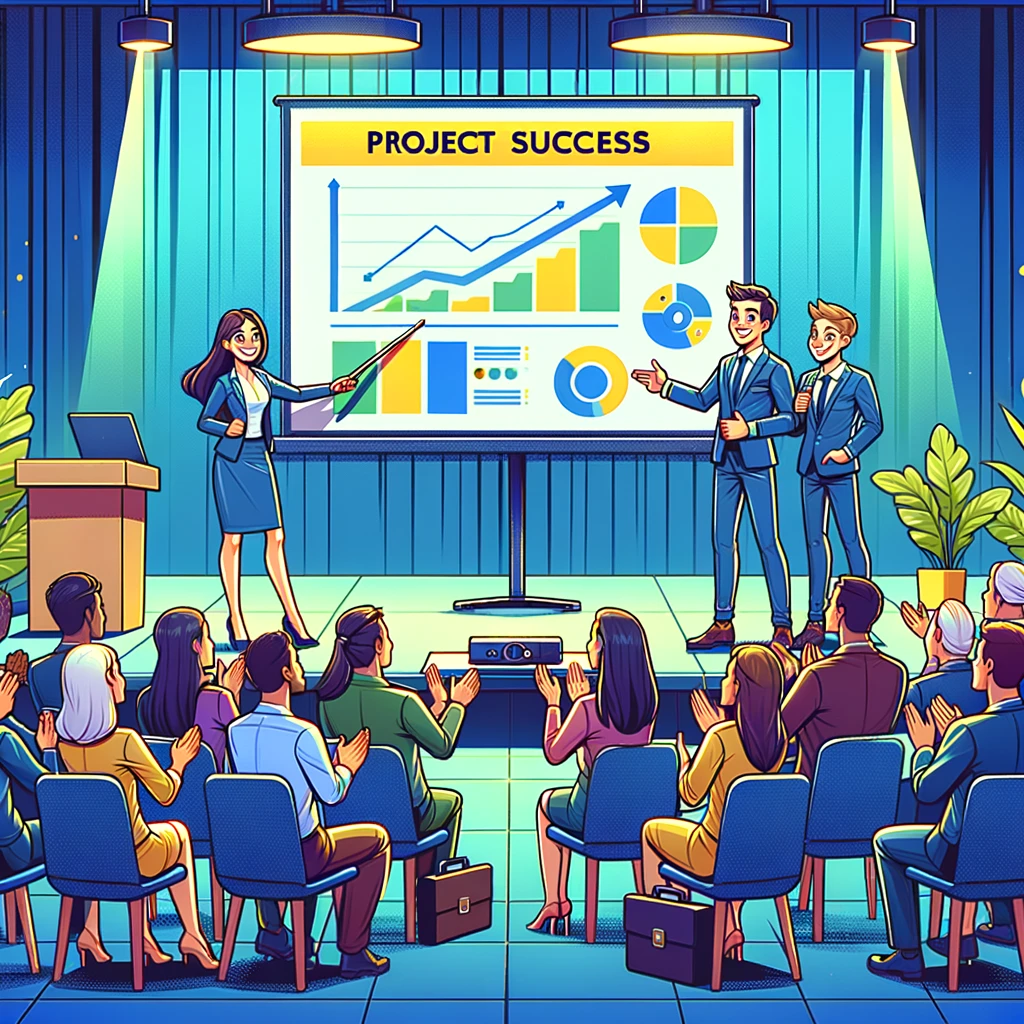
\includegraphics[width=0.9\textwidth]{day4}
    \end{figure}
    \end{column}
  \end{columns}
\end{frame}

\section{Rules}

\begin{frame}
  \frametitle{Rules for the Hackathon}
  \begin{columns}
    \begin{column}{0.5\textwidth}
      \begin{itemize}
      \item play fair!
      \item only use data provided in your challenge
      \item do not use other groups results
      \item use only the computation time you need
      \item do not use more presentation time as everyone else
      \item discuss publication with mentor and project mentor
      \end{itemize}
    \end{column}
    \begin{column}{0.5\textwidth}
    \begin{figure}
      
\includegraphics[width=0.9\textwidth]{rules}
    \end{figure}
    \end{column}
  \end{columns}
\end{frame}

\section*{Thank you for your attention!}
\renewcommand\Switch{0}
\renewcommand\citationtext{}
\subsection*{Questions?}

\begin{frame}
  % \frametitle{Conclusion \& Outlook}

  \centering
  \Huge{Happy Hacking!}
\end{frame}
\beginbackup


\label{fr:appendix}
\appendix

% \begin{frame}[allowframebreaks,noframenumbering]
%   \frametitle{References}
%   \printbibliography
% \end{frame}

\section{Backup slides}

\section*{The End}
\renewcommand\citationtext{}
\backupend
\end{document}

%%% Local Variables:
%%% mode: latex
%%% TeX-master: t
%%% End:
